%!TEX root = documentation.tex

\chapter{Master}

\section{About the Master} % (fold)
\label{sec:about_the_master}

The master is written Java and uses the JAMod Library for the communication with the sensors over the modbus protocoll. The view is created with the SWT Library. 
It's seperated in several parts:
\begin{itemize}
	\item View (see \ref{sec:view})
	\item Configuration (see \ref{sec:configuration})
	\item Stations  (see \ref{sec:stations})
	\item History (see \ref{sec:history})
\end{itemize}

It's needed to create a configuration file before collection process of the measurement values could be started. A sensor must be added to the master befor it can be used. Each sensor has a individual name and ip address and it's refered as a station. In the configuration phase it's nesseary to specify the kind of data that the stations collect. The data that is transfered from the station to the master is called Input Parameter. To configure the sensor it's possible to define configuration Parameters. These values are transfered from the master to the sensor. To map the parameters to the memory in the station they must be bound to addresses. This happens individually for each station. So it's possible to collect different data from different stations. It's also possible to configure the kind of plots that are generated (see \ref{sub:plots}).

After the configuration of the stations the collection process could be started. Each station is polled in its own thread. One collector thread collects the data from all stations, generates a text file with the information about the current values from the stations and draws the plots. The time between the polling of the stations and between generation of the output files can also be configured. As soon the current day changes the values from the last day are aggregated to a history value. This daily history is kept for one year. The values from the station are kept for two days so it's possible to plot hourly data. 

% section about_the_master (end)

\section{View} % (fold)
\label{sec:view}

The view is created with the help of SWT ( http://www.eclipse.org/swt/ ). SWT uses the os drawing apis to draw the widgets. So the look and feel of the application is very good integrated into the os it runs in. 

\subsection{Screenshots} % (fold)
\label{sub:screenshots}

\begin{figure}[ht]
    \centering
    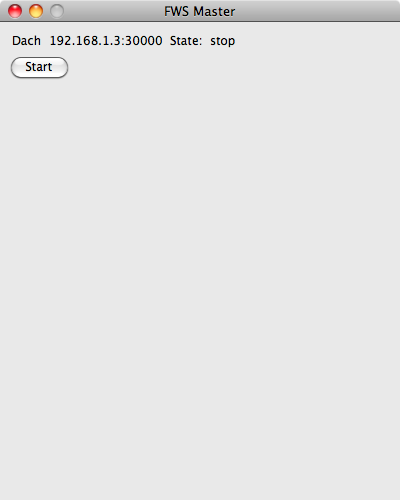
\includegraphics[width=0.6\linewidth]{master/mainview.png}
    \caption{Quick overview about the stations and their status}
    \label{fig:main}
\end{figure}

\begin{figure}[ht]
    \centering
    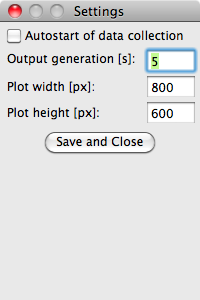
\includegraphics[width=0.4\linewidth]{master/settings.png}
    \caption{Configuration of the basic settings}
    \label{fig:settings}
\end{figure}

\begin{figure}[ht]
    \centering
    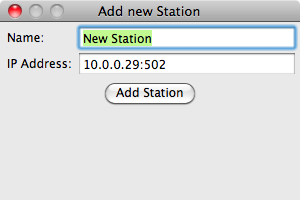
\includegraphics[width=0.6\linewidth]{master/add.png}
    \caption{Adds a new station to the master}
    \label{fig:add}
\end{figure}

% TODO bilder mit sinnvoller config einfügen
%\begin{figure}[ht]
%    \centering
%    \includegraphics[width=0.8\linewidth]{master/parameter.png}
%    \caption{Adding/editing of the parameters}
%    \label{fig:parameter}
%\end{figure}

%\begin{figure}[ht]
%    \centering
%    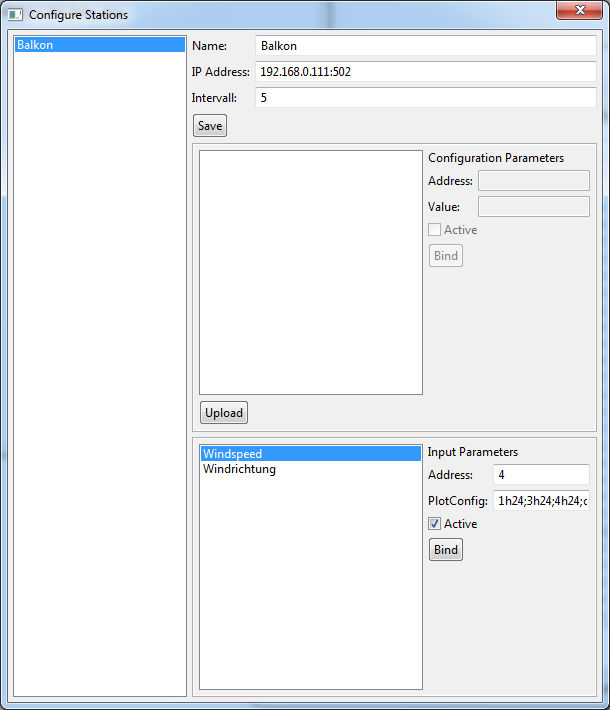
\includegraphics[width=0.8\linewidth]{master/stations.png}
%    \caption{Editing station specific settings. The parameters bindings are also set here}
%    \label{fig:stations}
%\end{figure}
%
%\begin{figure}[ht]
%    \centering
%    \includegraphics[width=0.8\linewidth]{master/data.png}
%    \caption{Shows the currently collected and saved data}
%    \label{fig:data}
%\end{figure}
% subsection screenshots (end)

\section{Configuration} % (fold)
\label{sec:configuration} 
%TODO enabled wenn vorhanden
The nessesary views for the configuration are \ref{fig:add}, \ref{fig:settings}, %\ref{fig:parameters} and \ref{fig:stations}.

The result of the configuration phase is an xml file with all settings in it. See example in Listing \ref{code:settings}

{\C \lstinputlisting[language=xml,breaklines=true,caption={Sample settings file},label=code:settings,frame=tlRB]{master/settings.xml} }

\subsection{Parameters} % (fold)
\label{sub:parameters}
There are two types of parameters. Input Parameters and Configuraton Parameters. Each parameters has a unique name and a boolean value if it's enabled. The name is the identifyer of the parameters so it has to be unique. Beside of these common attributes the configuration and input parameters have further attributes.

Additional attributes of an input parameter:

Additional attributes of a configuration parameter:

% subsection parameters (end)

\subsection{Plots} % (fold)
\label{sub:plots}
About the plots
% subsection plots (end)
% section configuration (end)

\section{Stations} % (fold)
\label{sec:stations}

% section stations (end)

\section{History} % (fold)
\label{sec:history}

% section history (end)